\chapter{Teori Medan Ligan dan Warna}\label{ch:b2:ligand-field}

Rubi berwarna merah dan zamrud hijau, namun keduanya berutang warna kepada
ion yang sama, \ce{Cr^3+}, yang sejumlah kecilnya menggantikan aluminium
dalam korundum, \ce{Al2O3}, atau dalam beril. Kristal tembaga sulfat
berwarna biru tua, tetapi serbuk yang tersisa setelah kristal itu dipanaskan
berwarna putih. Dalam setiap kasus, warna itu berasal dari elektron yang
melompat di antara orbital-orbital d yang energinya telah dipisahkan oleh
atom-atom di sekitarnya --- sebesar nilai yang bergantung pada atom mana
yang mengelilingi ion itu dan bagaimana caranya. Bab ini menghitung
pemisahan itu, mula-mula dengan muatan titik, kemudian dengan \omterm{def:b2:diatomic-mos:lcao}{orbital
molekul}; bab ini menjelaskan warna, kemagnetan, dan \omterm{def:b2:coordination-complexes:electron-count}{aturan 18 elektron} dari
bab sebelumnya.

\begin{recall}
\Cref{ch:b2:coordination-complexes}: konfigurasi $d^n$, geometri, jumlah
elektron. \Cref{ch:b2:atomic-orbitals}: bentuk kelima orbital d.
\Cref{ch:b2:fragment-orbitals}: \omterm{def:b2:fragment-orbitals:fragment}{orbital fragmen}. Jilid Tahun 1: absorbans,
warna komplementer, elektron tak berpasangan, aturan Hund.
\end{recall}

\begin{omfigure}
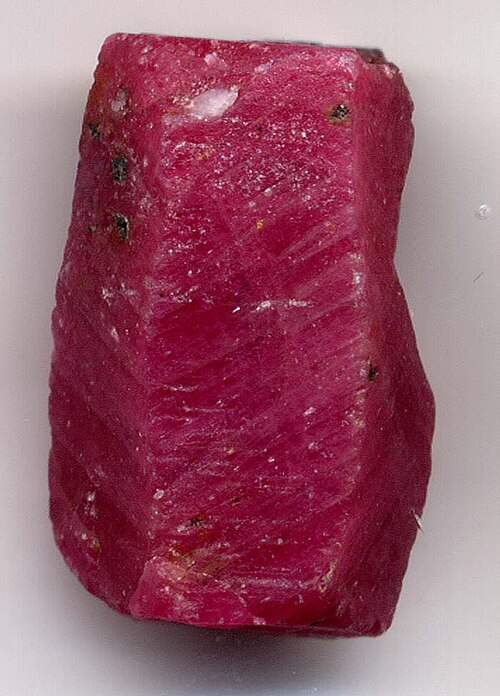
\includegraphics[height=3.6cm]{images/book3/ruby.jpg}\hspace{0.6cm}%
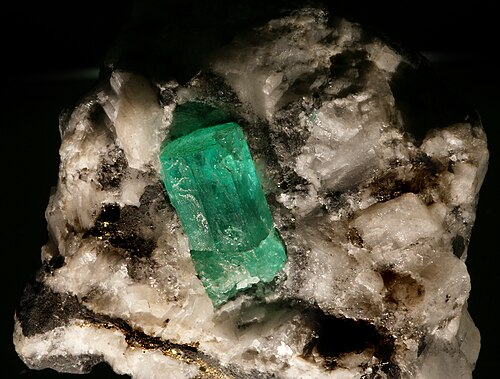
\includegraphics[height=3.6cm]{images/book3/emerald.jpg}\hspace{0.6cm}%
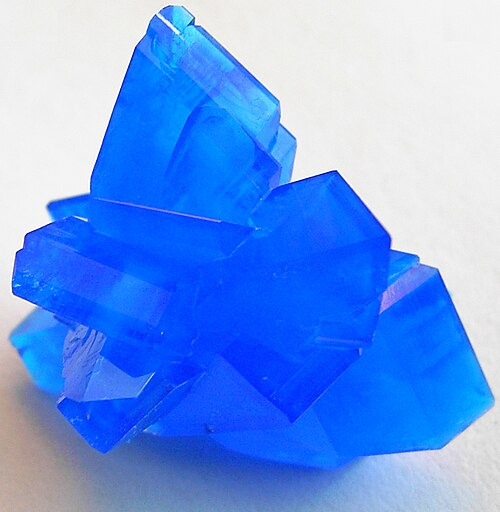
\includegraphics[height=3.6cm]{images/book3/copper-sulfate.jpg}

{\small Sebuah kristal rubi (domain publik); zamrud di dalam batuannya
(Didier Descouens, CC BY-SA 3.0); kristal tembaga(II) sulfat pentahidrat
(Stephanb, CC BY-SA 3.0). Wikimedia Commons. Kromium(III) mewarnai kedua
yang pertama, kompleks akua tembaga(II) yang ketiga.}
\end{omfigure}

\section{Model medan kristal}

\begin{definition}[Medan kristal]\label{def:b2:ligand-field:crystal-field}
Yang disebut \emph{model medan kristal}\index{model medan kristal}
memperlakukan ligan-ligan sebuah kompleks sebagai muatan titik negatif
(atau ujung negatif dipol) di sekeliling ion logam, dan menghitung bagaimana
ligan-ligan itu mengubah energi orbital-orbital d-nya. Dalam medan
oktahedral, orbital-orbital d terpisah menjadi dua himpunan yang berjarak
sebesar \emph{pemisahan medan kristal}\index{pemisahan medan kristal} $\Delta_o$.
\end{definition}

Letakkan keenam ligan pada sumbu-sumbu. Orbital $\mathrm d_{z^2}$ dan $\mathrm d_{x^2-y^2}$
mengarahkan cuping-cupingnya tepat ke ligan: elektron di dalamnya lebih
ditolak, dan orbital-orbital itu naik. Orbital $\mathrm d_{xy}$, $\mathrm d_{xz}$, $\mathrm d_{yz}$
mengarah di antara ligan-ligan dan naik lebih sedikit. Pasangan pertama
disebut $e_g$, himpunan kedua yang beranggota tiga
$t_{2g}$ (nama-nama dari teori grup, dalam jilid Tahun 3).

\begin{omfigure}
\begin{tikzpicture}[font=\small]
  \begin{scope}
    \pic at (0,0) {omdx2y2};
    \foreach \p in {(1.25,0),(-1.25,0),(0,1.25),(0,-1.25)} \node[circle, fill=black!70, inner sep=2.2pt] at \p {};
    \node at (0,-1.75) {$\mathrm d_{x^2-y^2}$: cuping ke arah ligan};
  \end{scope}
  \begin{scope}[xshift=5.5cm]
    \pic at (0,0) {omdxy};
    \foreach \p in {(1.25,0),(-1.25,0),(0,1.25),(0,-1.25)} \node[circle, fill=black!70, inner sep=2.2pt] at \p {};
    \node at (0,-1.75) {$\mathrm d_{xy}$: cuping di antara ligan};
  \end{scope}
\end{tikzpicture}

{\small Dua orbital d di antara keempat ligan pada bidang $xy$ sebuah
oktahedron (titik-titik hitam). Cuping-cuping $\mathrm d_{x^2-y^2}$ mengarah ke
ligan, cuping-cuping $\mathrm d_{xy}$ di antaranya.}
\end{omfigure}

\begin{theorem}[Barisentrum]\label{thm:b2:ligand-field:barycentre}
Dalam medan oktahedral, diukur dari energi rata-rata orbital-orbital d,
pasangan $e_g$ terletak pada $+0.6\Delta_o$ dan himpunan $t_{2g}$ pada $-0.4\Delta_o$.
\end{theorem}

\begin{proof}
Medan itu menaikkan rata-rata kelima energi d tetapi tidak mengubahnya
melalui pemisahan (aturan barisentrum, diterima tanpa bukti: jumlah
pergeseran sehimpunan orbital yang lengkap ditentukan oleh muatan total,
bukan oleh susunannya). Dengan $e_g$ pada $x$ dan
$t_{2g}$ pada $x - \Delta_o$, syarat $2x + 3(x - \Delta_o) = 0$ memberikan $x = 0.6\Delta_o$.
\end{proof}

\section{Spin tinggi dan spin rendah}

\begin{definition}[Keadaan spin]\label{def:b2:ligand-field:spin}
Yang disebut \emph{energi pemasangan}\index{energi pemasangan} $P$ adalah
energi yang diperlukan untuk menempatkan elektron kedua ke dalam orbital
yang sudah terisi alih-alih ke dalam orbital kosong yang berenergi sama.
Sebuah kompleks disebut \emph{spin tinggi}\index{spin tinggi} jika
elektron-elektronnya menempati orbital $e_g$ sebelum berpasangan dalam
$t_{2g}$, dan \emph{spin rendah}\index{spin rendah} jika
elektron-elektronnya berpasangan dalam $t_{2g}$ lebih dahulu.
\end{definition}

\begin{proposition}[Pilihan keadaan spin]\label{prop:b2:ligand-field:spin-state}
Untuk ion-ion oktahedral $d^4$ sampai $d^7$, kompleksnya berspin rendah jika
$\Delta_o > P$ dan berspin tinggi jika $\Delta_o < P$. Untuk $d^1$--$d^3$ dan
$d^8$--$d^{10}$ hanya ada satu konfigurasi.
\end{proposition}

\begin{proof}
Mulai dari $d^3$ ($t_{2g}^3$), elektron keempat masuk ke $e_g$ (biaya $\Delta_o$ di atas
$t_{2g}$) atau berpasangan dalam $t_{2g}$ (biaya $P$). Yang lebih murah
menang; perbandingan yang sama berlaku untuk setiap elektron sampai $d^7$.
Untuk $d^1$--$d^3$ masih ada tempat dalam $t_{2g}$ tanpa berpasangan;
untuk $d^8$--$d^{10}$, $t_{2g}$ penuh dan $e_g$ harus dipakai bagaimanapun juga.
\end{proof}

\begin{definition}[Energi stabilisasi medan kristal]\label{def:b2:ligand-field:cfse}
Yang disebut \emph{energi stabilisasi medan kristal}\index{energi stabilisasi medan kristal}
(CFSE) sebuah konfigurasi $t_{2g}^ae_g^b$ adalah $(-0.4a + 0.6b)\Delta_o$, yaitu
energi elektron-elektron d relatif terhadap barisentrum (\omterm{def:b2:ligand-field:spin}{energi pemasangan}
dihitung tersendiri).
\end{definition}

\begin{proposition}[CFSE sepanjang deret]\label{prop:b2:ligand-field:cfse}
Pada \omterm{def:b2:ligand-field:spin}{spin tinggi}, CFSE bernilai $0$, $-0.4$, $-0.8$, $-1.2$, $-0.6$, $0$, $-0.4$, $-0.8$, $-1.2$,
$-0.6$, $0$ (dalam $\Delta_o$) untuk $d^0$ sampai $d^{10}$: nilainya nol untuk $d^0$,
$d^5$, $d^{10}$. Pada \omterm{def:b2:ligand-field:spin}{spin rendah}, nilainya mencapai $-2.4\Delta_o$ untuk $d^6$.
\end{proposition}

\begin{proof}
Isilah konfigurasi-konfigurasinya dan terapkan definisinya; nilai-nilainya
adalah nilai-nilai pada gambar, yang dihitung.
\end{proof}

\begin{omfigure}
\begin{tikzpicture}
\begin{axis}[width=0.55\linewidth, height=5cm, xmin=-0.5, xmax=10.5, ymin=-2.6, ymax=0.3,
  axis x line=bottom, axis y line=left, xlabel={$d^n$}, ylabel={CFSE ($\Delta_o$)},
  xtick={0,1,2,3,4,5,6,7,8,9,10}, tick label style={font=\small}, label style={font=\small}]
\addplot[omThm, thick, mark=*, mark size=1.3pt] table[x=n, y=high] {figdata/out/bachelor-2-ligand-field-a.dat};
\addplot[omDef, thick, dashed, mark=square*, mark size=1.3pt] table[x=n, y=low] {figdata/out/bachelor-2-ligand-field-a.dat};
\node[font=\scriptsize, omThm, anchor=west] at (axis cs:5.4,0.0) {spin tinggi};
\node[font=\scriptsize, omDef, anchor=west] at (axis cs:6.6,-2.2) {spin rendah};
\end{axis}
\end{tikzpicture}\hfill
\begin{tikzpicture}[font=\small]
  \pic (t) at (0,0) {omlevel={ud}{0.5}}; \pic at (0.6,0) {omlevel={u}{0.5}}; \pic at (1.2,0) {omlevel={u}{0.5}};
  \pic at (0.3,1.6) {omlevel={u}{0.5}}; \pic at (0.9,1.6) {omlevel={u}{0.5}};
  \node at (0.6,-0.8) {$d^6$ spin tinggi};
  \node[font=\scriptsize, anchor=east] at (-0.35,0) {$t_{2g}$}; \node[font=\scriptsize, anchor=east] at (-0.05,1.6) {$e_g$};
  \pic at (3,0) {omlevel={ud}{0.5}}; \pic at (3.6,0) {omlevel={ud}{0.5}}; \pic at (4.2,0) {omlevel={ud}{0.5}};
  \pic at (3.3,2.4) {omlevel={empty}{0.5}}; \pic at (3.9,2.4) {omlevel={empty}{0.5}};
  \node at (3.6,-0.8) {$d^6$ spin rendah};
  \draw[<->, omProp] (4.7,0) -- (4.7,2.4) node[midway, right, font=\scriptsize] {$\Delta_o$};
  \draw[<->, omProp] (1.7,0) -- (1.7,1.6) node[midway, right, font=\scriptsize] {$\Delta_o$};
\end{tikzpicture}

{\small Kiri: \omterm{def:b2:ligand-field:cfse}{energi stabilisasi medan kristal} sepanjang deret d (dihitung),
\omterm{def:b2:ligand-field:spin}{spin tinggi} (garis penuh) dan \omterm{def:b2:ligand-field:spin}{spin rendah} (putus-putus). Kanan: kedua
konfigurasi sebuah ion $d^6$: empat elektron tak berpasangan jika $\Delta_o < P$
(seperti \ce{[Fe(H2O)6]^2+}), tidak ada jika $\Delta_o >
P$ (seperti \ce{[Fe(CN)6]^4-}).}
\end{omfigure}

\begin{method}[Keadaan spin, CFSE, dan elektron tak berpasangan]\label{met:b2:ligand-field:spin-state}
\begin{enumerate}
  \item Tentukan $n$ dari bilangan oksidasinya ($n = g - m$).
  \item Untuk $d^4$--$d^7$, bandingkan $\Delta_o$ dan $P$ (atau letakkan
        ligannya dalam \omterm{def:b2:ligand-field:spectrochemical}{deret spektrokimia}): medan kuat, \omterm{def:b2:ligand-field:spin}{spin rendah}; medan
        lemah, \omterm{def:b2:ligand-field:spin}{spin tinggi}.
  \item Isilah $t_{2g}$ dan $e_g$ sesuai dengan itu; CFSE $= (-0.4a + 0.6b)\Delta_o$.
  \item Hitunglah elektron tak berpasangan; satu saja elektron tak
        berpasangan membuat kompleks itu \omterm{def:b2:diatomic-mos:magnetism}{paramagnetik}.
\end{enumerate}
\end{method}

\section{Geometri lain}

\begin{proposition}[Medan tetrahedral dan bujur sangkar planar]\label{prop:b2:ligand-field:tetrahedral}
Dalam medan tetrahedral urutannya terbalik: dua orbital ($e$) di bawah tiga ($t_2$),
dengan pemisahan $\Delta_t \approx \frac49\Delta_o$ untuk logam dan ligan yang
sama; kompleks tetrahedral berspin tinggi. Dalam medan bujur sangkar planar
orbital $\mathrm d_{x^2-y^2}$ terletak jauh di atas yang lain: ion $d^8$
mengisi keempat orbital yang lebih rendah dan membiarkan orbital itu kosong.
\end{proposition}

\admitted

Faktor $4/9$ berasal dari geometri muatan-muatan titik; dengan hanya empat
ligan, yang tidak satu pun mengarah sepanjang sumbu, pemisahannya terlalu
kecil untuk mengatasi \omterm{def:b2:ligand-field:spin}{energi pemasangan}. Menyingkirkan kedua ligan pada
sumbu $z$ sebuah oktahedron menurunkan orbital-orbital yang mempunyai
komponen $z$ dan tidak menaikkan apa pun: inilah penjelasan kompleks-kompleks
$d^8$ bujur sangkar planar pada bab sebelumnya, yang kedelapan elektronnya
semua mendapat tempat di bawah $\mathrm d_{x^2-y^2}$ yang kosong.

\begin{omfigure}
\begin{tikzpicture}[font=\scriptsize]
  % octahedral
  \pic at (-0.3,0) {omlevel={empty}{0.45}}; \pic at (0.25,0) {omlevel={empty}{0.45}}; \pic at (0.8,0) {omlevel={empty}{0.45}};
  \pic at (0,1.8) {omlevel={empty}{0.45}}; \pic at (0.55,1.8) {omlevel={empty}{0.45}};
  \node[anchor=west] at (1.1,0) {$t_{2g}$}; \node[anchor=west] at (0.85,1.8) {$e_g$};
  \node[font=\small] at (0.25,-0.7) {oktahedral};
  % tetrahedral
  \begin{scope}[xshift=3.5cm]
    \pic at (0,0.6) {omlevel={empty}{0.45}}; \pic at (0.55,0.6) {omlevel={empty}{0.45}};
    \pic at (-0.3,1.4) {omlevel={empty}{0.45}}; \pic at (0.25,1.4) {omlevel={empty}{0.45}}; \pic at (0.8,1.4) {omlevel={empty}{0.45}};
    \node[anchor=west] at (0.85,0.6) {$e$}; \node[anchor=west] at (1.1,1.4) {$t_2$};
    \node[font=\small] at (0.25,-0.7) {tetrahedral};
  \end{scope}
  % square planar
  \begin{scope}[xshift=7cm]
    \pic at (0,-0.2) {omlevel={empty}{0.45}}; \pic at (0.55,-0.2) {omlevel={empty}{0.45}};
    \pic at (0.25,0.3) {omlevel={empty}{0.45}};
    \pic at (0.25,0.9) {omlevel={empty}{0.45}};
    \pic at (0.25,2.6) {omlevel={empty}{0.45}};
    \node[anchor=west] at (0.85,-0.2) {$\mathrm d_{xz}, \mathrm d_{yz}$};
    \node[anchor=west] at (0.55,0.3) {$\mathrm d_{z^2}$};
    \node[anchor=west] at (0.55,0.9) {$\mathrm d_{xy}$};
    \node[anchor=west] at (0.55,2.6) {$\mathrm d_{x^2-y^2}$};
    \node[font=\small] at (0.25,-0.7) {bujur sangkar planar};
  \end{scope}
\end{tikzpicture}

{\small Pemisahan orbital-orbital d dalam tiga geometri, skematis (tidak
dengan skala yang sama): oktahedral, tetrahedral (terbalik dan lebih
kecil), bujur sangkar planar (satu orbital jauh di atas yang lain).}
\end{omfigure}

\section{Warna dan deret spektrokimia}

\begin{definition}[Transisi d--d]\label{def:b2:ligand-field:d-d}
Yang disebut \emph{transisi d--d}\index{transisi d--d} adalah promosi sebuah
elektron dari tingkat d yang lebih rendah ke tingkat d yang lebih tinggi
dalam sebuah kompleks melalui penyerapan cahaya; untuk ion $d^1$, dari
$t_{2g}$ ke $e_g$, pada energi $\Delta_o$.
\end{definition}

\begin{proposition}[Pemisahan dari warna]\label{prop:b2:ligand-field:colour}
Jika sebuah kompleks menyerap paling kuat pada panjang gelombang
$\lambda_{\max}$ melalui \omterm{def:b2:ligand-field:d-d}{transisi d--d} berenergi $\Delta_o$, maka
$\Delta_o = N_Ahc/\lambda_{\max}$ per mol, atau $\tilde\nu = 1/\lambda_{\max}$ dalam
bilangan gelombang; warna yang terlihat adalah komplemen warna yang diserap.
\end{proposition}

\begin{proof}
Sebuah foton berpanjang gelombang $\lambda$ membawa $hc/\lambda$; satu mol foton, $N_Ahc/\lambda$.
Cahaya putih dikurangi pita yang diserap tampak dalam warna komplementernya.
\end{proof}

\begin{method}[Dari pita serapan ke warna]\label{met:b2:ligand-field:colour}
\begin{enumerate}
  \item Ubahlah $\lambda_{\max}$ menjadi $\tilde\nu = 1/\lambda_{\max}$ (\unit{cm^{-1}}) dan menjadi
        $N_Ahc/\lambda_{\max}$ (\unit{kJ/mol}): $\qty{500}{nm} \leftrightarrow \qty{20000}{cm^{-1}}
        \leftrightarrow \qty{239}{kJ/mol}$.
  \item Tentukan warna yang diserap (ungu 400--430, biru 430--490, hijau
        490--560, kuning 560--590, jingga 590--620, merah 620--700 nm, kira-kira).
  \item Warna yang terlihat terletak di seberangnya pada roda warna.
\end{enumerate}
\end{method}

\begin{omfigure}
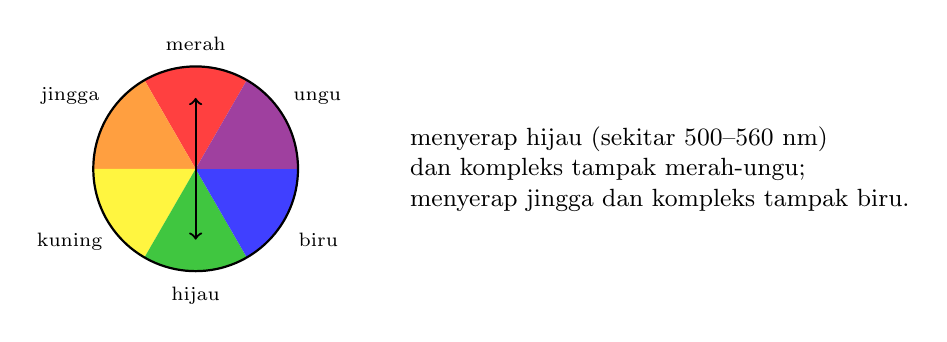
\begin{tikzpicture}[font=\scriptsize]
  \foreach \a/\c/\n in {90/red/merah, 150/orange/jingga, 210/yellow/kuning, 270/green!70!black/hijau, 330/blue/biru, 30/violet/ungu} {
    \fill[\c!75] (0,0) -- (\a-30:1.3) arc[start angle=\a-30, end angle=\a+30, radius=1.3] -- cycle;
    \node[anchor=\a+180] at (\a:1.38) {\n};
  }
  \draw[thick] (0,0) circle (1.3);
  \draw[<->, thick] (90:0.9) -- (270:0.9);
  \node[anchor=west, font=\small, align=left] at (2.6,0) {menyerap hijau (sekitar 500--560 nm)\\ dan kompleks tampak merah-ungu;\\ menyerap jingga dan kompleks tampak biru.};
\end{tikzpicture}

{\small Sebuah roda warna: warna yang terlihat kira-kira adalah komplemen,
yang berseberangan secara diametral, dari pita yang diserap.}
\end{omfigure}

\begin{definition}[Deret spektrokimia]\label{def:b2:ligand-field:spectrochemical}
Yang disebut \emph{deret spektrokimia}\index{deret spektrokimia} mengurutkan
ligan-ligan menurut pemisahan yang dihasilkannya untuk suatu ion logam
tertentu:
\[
  \ce{I-} < \ce{Br-} < \ce{Cl-} < \ce{F-} < \ce{OH-} < \ce{H2O} < \ce{NH3} < \text{en} <
  \ce{NO2-} < \ce{CN-} < \ce{CO} .
\]
Untuk ligan tertentu, $\Delta_o$ juga bertambah seiring muatan ion logam dan
ke bawah dalam satu golongan (kompleks 4d dan 5d, yang lebih besar daripada
3d, hampir selalu berspin rendah).
\end{definition}

Halida berada di ujung lemah dan \ce{CN-} serta \ce{CO} di ujung kuat, yang
tidak dapat dijelaskan oleh \omterm{def:b2:ligand-field:crystal-field}{model medan kristal}: model itu akan menempatkan
\ce{F-} yang bermuatan di atas \ce{CO} yang netral. Penjelasannya
memerlukan orbital.

\section{Medan ligan}

\begin{definition}[Teori medan ligan]\label{def:b2:ligand-field:ligand-field}
Yang disebut \emph{teori medan ligan}\index{teori medan ligan} menggambarkan
sebuah kompleks dengan orbital-orbital molekul yang dibangun dari
orbital-orbital valensi logam (kesembilan orbital $n$d, $(n+1)$s, dan $(n+1)$p-nya)
dan orbital-orbital donor ligan.
\end{definition}

\begin{proposition}[Ikatan $\sigma$ dalam kompleks oktahedral]\label{prop:b2:ligand-field:mo-octahedral}
Dengan enam ligan yang masing-masing memberikan satu orbital donor $\sigma$,
enam \omterm{def:b2:diatomic-mos:lcao}{orbital molekul} ikatan terbentuk dari orbital s, ketiga p, dan kedua
orbital d $e_g$ logam; ketiga orbital $t_{2g}$, yang mengarah di antara
ligan-ligan, tetap nonikatan; di atasnya terletak orbital-orbital antiikatan
$e_g^*$. Elektron-elektron ligan mengisi keenam \omterm{def:b2:diatomic-mos:bonding}{orbital ikatan}; elektron-elektron
d logam masuk ke $t_{2g}$ dan $e_g^*$, yang berjarak $\Delta_o$. \omterm{def:b2:diatomic-mos:bonding}{Orbital ikatan}
ditambah \omterm{def:b2:diatomic-mos:bonding}{orbital nonikatan} dapat menampung
$12 + 6 = 18$ elektron.
\end{proposition}

\begin{proof}[Argumen]
Dengan metode fragmen pada \cref{ch:b2:fragment-orbitals}, setiap orbital
logam berinteraksi dengan kombinasi orbital-orbital ligan yang bersimetri
sama: s dengan kombinasi yang simetris sepenuhnya, setiap p dengan sepasang
ligan yang berseberangan, $\mathrm d_{z^2}$ dan $\mathrm
d_{x^2-y^2}$ dengan kombinasi-kombinasi yang mengarah sepanjang
cuping-cupingnya; tidak ada kombinasi $\sigma$ yang cocok dengan orbital-orbital
$t_{2g}$ (tumpang-tindihnya dengan donor $\sigma$ mana pun yang mengarah
sepanjang sumbu bernilai nol karena simetri). Nama-nama kombinasi itu
berasal dari teori grup, diterima tanpa bukti. Mengisi semua \omterm{def:b2:diatomic-mos:bonding}{orbital ikatan}
dan nonikatan, dan tidak satu pun \omterm{def:b2:diatomic-mos:bonding}{orbital antiikatan}, memerlukan 18
elektron --- \omterm{def:b2:coordination-complexes:electron-count}{aturan 18 elektron}.
\end{proof}

\begin{omfigure}
\begin{tikzpicture}[font=\scriptsize]
  % metal
  \pic (m4p1) at (-0.45,2.6) {omlevel={empty}{0.4}}; \pic (m4p2) at (0,2.6) {omlevel={empty}{0.4}}; \pic (m4p3) at (0.45,2.6) {omlevel={empty}{0.4}};
  \node[anchor=east] at (-0.7,2.6) {$(n{+}1)$p};
  \pic (m4s) at (0,1.8) {omlevel={empty}{0.6}}; \node[anchor=east] at (-0.35,1.8) {$(n{+}1)$s};
  \foreach \x in {-0.9,-0.45,0,0.45,0.9} \pic at (\x,0.6) {omlevel={empty}{0.4}};
  \coordinate (m3d) at (1.1,0.6); \node[anchor=east] at (-1.15,0.6) {$n$d};
  \node[font=\small] at (0,-2.9) {logam};
  % ligands
  \foreach \x in {6.2,6.72,7.24,7.76,8.28,8.8} \pic at (\x,-0.9) {omlevel={ud}{0.36}};
  \coordinate (lig) at (6.0,-0.9);
  \node[font=\small] at (7.3,-2.9) {enam orbital donor $\sigma$};
  % MOs
  \pic (b1) at (3.6,-2.4) {omlevel={ud}{0.5}};
  \foreach \x in {3.0,3.6,4.2} \pic at (\x,-1.9) {omlevel={ud}{0.5}};
  \pic at (3.3,-1.45) {omlevel={ud}{0.5}}; \pic at (3.9,-1.45) {omlevel={ud}{0.5}};
  \foreach \x in {3.0,3.6,4.2} \pic at (\x,0.3) {omlevel={empty}{0.5}};
  \pic at (3.3,1.5) {omlevel={empty}{0.5}}; \pic at (3.9,1.5) {omlevel={empty}{0.5}};
  \pic at (3.6,3.1) {omlevel={empty}{0.5}};
  \foreach \x in {3.0,3.6,4.2} \pic at (\x,3.6) {omlevel={empty}{0.5}};
  \node[anchor=north] at (3.6,0.12) {$t_{2g}$ (nonikatan)};
  \node[anchor=west] at (4.2,1.5) {$e_g^*$};
  \node[anchor=north] at (3.6,-2.58) {6 ikatan};
  \draw[<->, omProp] (2.55,0.3) -- (2.55,1.5) node[midway, right] {$\Delta_o$};
  \draw[omcorr, densely dashed] (m3d) -- (2.75,0.3) (m3d) -- (3.05,1.5) (1.1,0.6) -- (3.05,-1.45);
  \draw[omcorr, densely dashed] (lig) -- (4.15,-1.45) (lig) -- (4.45,-1.9) (lig) -- (3.85,-2.4) (lig) -- (4.15,1.5);
  \draw[omcorr, densely dashed] (m4s-r) -- (3.35,-2.4) (m4s-r) -- (3.35,3.1) (m4p3-r) -- (2.75,-1.9) (m4p3-r) -- (2.75,3.6);
\end{tikzpicture}

{\small Orbital-orbital molekul sebuah kompleks oktahedral dengan enam donor
$\sigma$, skematis. Kedua belas elektron ligan mengisi keenam \omterm{def:b2:diatomic-mos:bonding}{orbital ikatan};
elektron-elektron d logam menempati tingkat $t_{2g}$ yang nonikatan dan
tingkat $e_g^*$ yang antiikatan, yang berjarak
$\Delta_o$ --- gambaran medan kristal diperoleh kembali. Sampai 18 elektron
mengisi tingkat-tingkat ikatan dan nonikatan.}
\end{omfigure}

\begin{definition}[Ligan donor $\pi$ dan akseptor $\pi$]\label{def:b2:ligand-field:pi-ligands}
Sebuah \emph{ligan donor $\pi$}\index{ligan donor pi@ligan donor $\pi$}
mempunyai orbital-orbital terisi yang bersimetri $\pi$ terhadap ikatan
logam--ligan (pasangan elektron bebas \ce{Cl-},
\ce{OH-}); sebuah \emph{ligan akseptor $\pi$}\index{ligan akseptor pi@ligan akseptor $\pi$}
mempunyai orbital-orbital kosong berenergi rendah (orbital $\pi^*$ \ce{CO} dan
\ce{CN-}). Perpindahan kerapatan elektron dari orbital-orbital d logam yang
terisi ke orbital-orbital $\pi^*$ kosong sebuah ligan
akseptor $\pi$ disebut \emph{donasi balik}\index{donasi balik}.
\end{definition}

\begin{proposition}[Efek $\pi$ pada pemisahan]\label{prop:b2:ligand-field:pi-effects}
Ligan donor $\pi$ memperkecil $\Delta_o$; ligan akseptor $\pi$ memperbesarnya.
\end{proposition}

\begin{proof}
Orbital-orbital $t_{2g}$ mempunyai simetri yang tepat untuk bertumpang-tindih
dengan orbital-orbital $\pi$ ligan. Orbital $\pi$ ligan yang terisi terletak
di bawah $t_{2g}$: menurut \cref{thm:b2:frontier-orbitals:perturbation},
interaksi itu mendorong $t_{2g}$ ke atas, ke arah $e_g^*$, dan $\Delta_o$ menyusut.
Orbital $\pi^*$ yang kosong terletak di atas $t_{2g}$: interaksi itu
mendorong $t_{2g}$ ke bawah, dan $\Delta_o$ membesar. Kasus kedua
memindahkan kerapatan d logam ke $\pi^*$ ligan: \omterm{def:b2:ligand-field:pi-ligands}{donasi balik}.
\end{proof}

\begin{omfigure}
\begin{tikzpicture}[font=\scriptsize]
  \begin{scope}
    \pic (t) at (0,1.2) {omlevel={empty}{0.6}}; \node[anchor=east] at (-0.35,1.2) {$t_{2g}$};
    \pic (l) at (2.4,0) {omlevel={ud}{0.6}}; \node[anchor=west] at (2.75,0) {$\pi$ ligan (terisi)};
    \pic (n) at (1.2,1.75) {omlevel={empty}{0.6}};
    \draw[omcorr, densely dashed] (t-r) -- (n-l) (l-l) -- (n-r);
    \pic (e) at (1.2,3.0) {omlevel={empty}{0.6}}; \node[anchor=west] at (1.55,3.0) {$e_g^*$};
    \draw[<->, omProp] (0.55,1.75) -- (0.55,3.0) node[midway, left] {$\Delta_o$ lebih kecil};
    \node[font=\small] at (1.2,-0.8) {donor $\pi$};
  \end{scope}
  \begin{scope}[xshift=6.5cm]
    \pic (t) at (0,1.2) {omlevel={empty}{0.6}}; \node[anchor=east] at (-0.35,1.2) {$t_{2g}$};
    \pic (l) at (2.4,2.6) {omlevel={empty}{0.6}}; \node[anchor=west] at (2.75,2.6) {$\pi^*$ ligan (kosong)};
    \pic (n) at (1.2,0.65) {omlevel={empty}{0.6}};
    \draw[omcorr, densely dashed] (t-r) -- (n-l) (l-l) -- (n-r);
    \pic (e) at (1.2,3.0) {omlevel={empty}{0.6}}; \node[anchor=west] at (1.55,3.15) {$e_g^*$};
    \draw[<->, omProp] (0.55,0.65) -- (0.55,3.0) node[midway, left] {$\Delta_o$ lebih besar};
    \node[font=\small] at (1.2,-0.8) {akseptor $\pi$ (donasi balik)};
  \end{scope}
\end{tikzpicture}

{\small Efek orbital-orbital $\pi$ ligan pada tingkat $t_{2g}$, skematis.
Orbital $\pi$ ligan yang terisi di bawahnya mendorong $t_{2g}$ ke atas
(pemisahan lebih kecil); orbital $\pi^*$ yang kosong di atasnya menariknya
ke bawah (pemisahan lebih besar).}
\end{omfigure}

Hal ini menempatkan \ce{CO} dan \ce{CN-}, donor $\sigma$ yang kuat sekaligus
akseptor $\pi$, di puncak \omterm{def:b2:ligand-field:spectrochemical}{deret spektrokimia}, dan halida, yang merupakan
donor $\pi$, di dasarnya. Orbital-orbital $t_{2g}$ karbonil logam
terstabilkan dan terisi: kompleks-kompleks 18 elektron pada
\cref{ch:b2:coordination-complexes}.

\section{Latihan}

\begin{exercise}[$\star$]\label{exo:b2:ligand-field:1}
Tuliskan konfigurasi oktahedral dan CFSE ion $d^3$ dan ion $d^8$.
\end{exercise}

\begin{exercise}[$\star$]\label{exo:b2:ligand-field:2}
Berapa elektron tak berpasangan yang dimiliki \ce{[Fe(H2O)6]^2+} (\omterm{def:b2:ligand-field:spin}{spin
tinggi}) dan \ce{[Fe(CN)6]^4-} (\omterm{def:b2:ligand-field:spin}{spin rendah})?
\end{exercise}

\begin{exercise}[$\star$]\label{exo:b2:ligand-field:3}
Sebuah kompleks menyerap paling kuat pada \qty{600}{nm}. Warna apakah yang tampak?
\end{exercise}

\begin{exercise}[$\star$]\label{exo:b2:ligand-field:4}
Urutkan \ce{H2O}, \ce{CN-}, \ce{Cl-}, \ce{NH3} menurut pemisahan yang dihasilkannya.
\end{exercise}

\begin{exercise}[$\star\star$]\label{exo:b2:ligand-field:5}
Untuk ion $d^5$, $\Delta_o = \qty{165}{kJ/mol}$ dengan air dan $\qty{390}{kJ/mol}$
dengan sianida, dan $P = \qty{300}{kJ/mol}$ (data latihan). Ramalkan kedua
keadaan spin dan elektron-elektron tak berpasangannya.
\end{exercise}

\begin{exercise}[$\star\star$]\label{exo:b2:ligand-field:6}
\ce{[Co(H2O)6]^2+} berwarna merah muda, \ce{[CoCl4]^2-} biru tua. Jelaskan
perubahan warna itu dari perubahan geometri dan ligannya.
\end{exercise}

\begin{exercise}[$\star\star$]\label{exo:b2:ligand-field:7}
Tunjukkan bahwa \ce{[Ni(CN)4]^2-} yang bujur sangkar planar bersifat
\omterm{def:b2:diatomic-mos:magnetism}{diamagnetik}, sedangkan \ce{[NiCl4]^2-} yang tetrahedral mempunyai dua
elektron tak berpasangan.
\end{exercise}

\begin{exercise}[$\star\star$]\label{exo:b2:ligand-field:8}
Sebuah kompleks $d^1$ menyerap pada \qty{500}{nm} (data latihan). Hitunglah
$\Delta_o$ dalam \unit{cm^{-1}} dan
\unit{kJ/mol}.
\end{exercise}

\begin{exercise}[$\star\star$]\label{exo:b2:ligand-field:9}
Mengapa senyawa-senyawa \ce{Zn^2+} dan \ce{Sc^3+} tidak berwarna?
\end{exercise}

\begin{exercise}[$\star\star\star$]\label{exo:b2:ligand-field:10}
Hitunglah elektron-elektron dalam orbital-orbital molekul \ce{[Co(NH3)6]^3+}:
tingkat-tingkat mana yang terisi, dan apakah kompleks itu \omterm{def:b2:diatomic-mos:magnetism}{diamagnetik}?
\end{exercise}

\begin{exercise}[$\star\star\star$]\label{exo:b2:ligand-field:11}
Jelaskan mengapa \ce{CO}, molekul netral yang bersifat basa lemah,
menghasilkan pemisahan yang lebih besar daripada ion fluorida.
\end{exercise}

\begin{exercise}[$\star\star\star$]\label{exo:b2:ligand-field:12}
Entalpi hidrasi ion-ion \ce{M^2+} dari \ce{Ca^2+} sampai \ce{Zn^2+}, yang
dialurkan terhadap $n$, membentuk dua punuk di atas garis lurus yang melalui
$d^0$, $d^5$, dan $d^{10}$. Jelaskan bentuk itu dengan CFSE \omterm{def:b2:ligand-field:spin}{spin tinggi}.
\end{exercise}

\section{Soal: Rubi Merah, Zamrud Hijau}

\begin{problem}[{Soal akhir pekan --- kromium(III) dalam medan oktahedral,
pita-pita serapan rubi dan warna yang ditinggalkannya, medan zamrud yang
lebih lemah, serta tembaga sulfat terhidrasi dan anhidrat}]
\label{pb:b2:ligand-field:1}
Data yang dinyatakan untuk soal ini (dibulatkan, ilustratif): rubi (\ce{Cr^3+}
dalam \ce{Al2O3}) menyerap dalam dua pita, di dekat \qty{556}{nm} dan
\qty{405}{nm}; dalam zamrud (\ce{Cr^3+} dalam beril) pita pertama terletak di
dekat \qty{620}{nm}. Untuk ion $d^3$, pita pertama bersesuaian dengan
$\Delta_o$. $N_Ahc = \qty{0.1196}{J.m/mol}$.
% ledger: const:NA, const:h, const:c

\medskip
\noindent\textbf{Bagian I --- Kromium(III).}
\begin{enumerate}
  \item Tuliskan konfigurasi $d^n$ \ce{Cr^3+}.
  \item Bagaimana konfigurasi itu tersebar dalam medan oktahedral?
  \item Apakah ada pilihan antara \omterm{def:b2:ligand-field:spin}{spin tinggi} dan \omterm{def:b2:ligand-field:spin}{spin rendah}?
  \item Hitunglah CFSE-nya.
  \item Berapa elektron tak berpasangan yang dimilikinya?
  \item Mengapa kompleks-kompleks kromium(III) inert secara kinetik (lambat
        menukar ligan)?
\end{enumerate}

\medskip
\noindent\textbf{Bagian II --- Rubi.}
\begin{enumerate}[resume]
  \item Apa yang mengelilingi ion \ce{Cr^3+} yang menggantikan \ce{Al^3+}
        dalam korundum?
  \item Ubahlah pita pertama menjadi bilangan gelombang.
  \item Simpulkan $\Delta_o$ dalam \unit{kJ/mol}.
  \item Warna-warna apakah yang diserap oleh kedua pita itu?
  \item Apa yang tersisa untuk dilihat?
  \item Mengapa ada dua pita untuk satu pemisahan saja? (Jawaban kualitatif.)
\end{enumerate}

\medskip
\noindent\textbf{Bagian III --- Zamrud.}
\begin{enumerate}[resume]
  \item Ubahlah pita zamrud menjadi $\Delta_o$.
  \item Bandingkan dengan rubi: kristal manakah yang memberikan medan yang lebih kuat?
  \item Ke mana warna yang diserap bergeser, dan warna apakah yang diteruskan?
  \item Usulkan alasan struktural untuk medan yang lebih lemah dalam beril.
  \item Apakah jumlah elektron tak berpasangan akan berubah?
\end{enumerate}

\medskip
\noindent\textbf{Bagian IV --- Tembaga sulfat.}
\begin{enumerate}[resume]
  \item Apa konfigurasi \ce{Cu^2+}?
  \item Dalam \ce{CuSO4.5H2O}, tembaga dikelilingi oleh molekul-molekul air.
        Mengapa padatan itu berwarna biru?
  \item Apa yang terjadi pada warnanya ketika airnya diusir, dan mengapa?
  \item Mengapa setetes air membuat serbuk putih itu biru kembali?
  \item Apakah \ce{[Cu(NH3)4]^2+} akan menyerap pada panjang gelombang yang
        lebih pendek atau lebih panjang daripada ion akuanya?
  \item Dapatkah ion $d^9$ berspin tinggi atau berspin rendah?
  \item Apakah \ce{CuSO4.5H2O} \omterm{def:b2:diatomic-mos:magnetism}{paramagnetik}?
  \item Nyatakan $\Delta_o$ \ce{Cr^3+} dalam rubi dari pita serapan pertamanya.
\end{enumerate}
\end{problem}
